\documentclass{article}\usepackage[]{graphicx}\usepackage[]{color}
%% maxwidth is the original width if it is less than linewidth
%% otherwise use linewidth (to make sure the graphics do not exceed the margin)
\makeatletter
\def\maxwidth{ %
  \ifdim\Gin@nat@width>\linewidth
    \linewidth
  \else
    \Gin@nat@width
  \fi
}
\makeatother

\definecolor{fgcolor}{rgb}{0.345, 0.345, 0.345}
\newcommand{\hlnum}[1]{\textcolor[rgb]{0.686,0.059,0.569}{#1}}%
\newcommand{\hlstr}[1]{\textcolor[rgb]{0.192,0.494,0.8}{#1}}%
\newcommand{\hlcom}[1]{\textcolor[rgb]{0.678,0.584,0.686}{\textit{#1}}}%
\newcommand{\hlopt}[1]{\textcolor[rgb]{0,0,0}{#1}}%
\newcommand{\hlstd}[1]{\textcolor[rgb]{0.345,0.345,0.345}{#1}}%
\newcommand{\hlkwa}[1]{\textcolor[rgb]{0.161,0.373,0.58}{\textbf{#1}}}%
\newcommand{\hlkwb}[1]{\textcolor[rgb]{0.69,0.353,0.396}{#1}}%
\newcommand{\hlkwc}[1]{\textcolor[rgb]{0.333,0.667,0.333}{#1}}%
\newcommand{\hlkwd}[1]{\textcolor[rgb]{0.737,0.353,0.396}{\textbf{#1}}}%
\let\hlipl\hlkwb

\usepackage{framed}
\makeatletter
\newenvironment{kframe}{%
 \def\at@end@of@kframe{}%
 \ifinner\ifhmode%
  \def\at@end@of@kframe{\end{minipage}}%
  \begin{minipage}{\columnwidth}%
 \fi\fi%
 \def\FrameCommand##1{\hskip\@totalleftmargin \hskip-\fboxsep
 \colorbox{shadecolor}{##1}\hskip-\fboxsep
     % There is no \\@totalrightmargin, so:
     \hskip-\linewidth \hskip-\@totalleftmargin \hskip\columnwidth}%
 \MakeFramed {\advance\hsize-\width
   \@totalleftmargin\z@ \linewidth\hsize
   \@setminipage}}%
 {\par\unskip\endMakeFramed%
 \at@end@of@kframe}
\makeatother

\definecolor{shadecolor}{rgb}{.97, .97, .97}
\definecolor{messagecolor}{rgb}{0, 0, 0}
\definecolor{warningcolor}{rgb}{1, 0, 1}
\definecolor{errorcolor}{rgb}{1, 0, 0}
\newenvironment{knitrout}{}{} % an empty environment to be redefined in TeX

\usepackage{alltt}

\usepackage{fancyhdr} % Required for custom headers
\usepackage{lastpage} % Required to determine the last page for the footer
\usepackage{extramarks} % Required for headers and footers
\usepackage{graphicx} % Required to insert images
\usepackage{hyperref}
\usepackage{amsmath} %for binomial pdf
\usepackage{parskip} % so that there's space bw paragraphs
\usepackage{float}
\usepackage{amsfonts}
\usepackage{verbatim}
\graphicspath{"~/almhub_0823/exp_design/homework/HW4"}



% Margins
\topmargin=-0.45in
\evensidemargin=0in
\oddsidemargin=0in
\textwidth=6.5in
\textheight=9.0in
\headsep=0.25in 

\linespread{1.1} % Line spacing

% Set up the header and footer
\pagestyle{fancy}
\lhead{STAT 541: Experimental Design} % Top left header
\chead{HW 6} % Top center header
\rhead{Andrea Mack} % Top right header
\lfoot{03/24/2017} % Bottom left footer
\cfoot{} % Bottom center footer
\rfoot{Page\ \thepage\ of\ \pageref{LastPage}} % Bottom right footer
\renewcommand\headrulewidth{0.4pt} % Size of the header rule
\renewcommand\footrulewidth{0.4pt} % Size of the footer rule

\setlength\parindent{0pt} % Removes all indentation from paragraphs
\setlength\parskip{0.5cm}
\restylefloat{table}

%----------------------------------------------------------------------------------------
%	DOCUMENT STRUCTURE COMMANDS
%	Skip this unless you know what you're doing
%----------------------------------------------------------------------------------------

% Header and footer for when a page split occurs within a problem environment
\newcommand{\enterProblemHeader}[1]{
\nobreak\extramarks{#1}{#1 continued on next page\ldots}\nobreak
\nobreak\extramarks{#1 (continued)}{#1 continued on next page\ldots}\nobreak
}

% Header and footer for when a page split occurs between problem environments
\newcommand{\exitProblemHeader}[1]{
\nobreak\extramarks{#1 (continued)}{#1 continued on next page\ldots}\nobreak
\nobreak\extramarks{#1}{}\nobreak
}


%----------------------------------------------------------------------------------------%
\IfFileExists{upquote.sty}{\usepackage{upquote}}{}
\begin{document}



\begin{enumerate}
\item %1

BIBD with b=14, a=8, k=4, r=7, and $\lambda$ = 3.

\begin{center}
\begin{tabular}{ |c|c|c|c|c|c|c|c|c|c|c|c|c|c|c|c| } 
 \hline
 &1&2&3&4&5&6&7&8&9&10&11&12&13&14\\ \hline
 1&x& &x&x&x&x&x& & & & & & &x\\ \hline 
  2&x& &x& &x& & &x& &x& &x&x& \\ \hline
   3&x&x& &x& &x& &x& &x&x& & & \\ \hline
   4&x&x& & & & &x&x&x& & & &x&x\\ \hline
     5& & &x&x& & & &x&x& &x&x& &x\\ \hline
      6& & & &x&x& &x& &x&x&x& &x& \\ \hline
       7& &x& & &x&x& & &x&x& &x& &x\\ \hline
        8& &x&x& & &x&x& & & &x&x&x& \\ \hline
\end{tabular}
\end{center}

\item %2
{\it Verify that a BIBD with the parameters a=8, r=8, k=4, and b=16 does not exist.}

$\lambda = \frac{r(k-1)}{(a-1)}$

$\rightarrow \lambda = \frac{8(4-1)}{(8-1)}$

$\rightarrow \lambda = \frac{24}{7}$

$\lambda$ must be an integer to have a valid BIBD, and so this set up for a BIBD does not exist.

\item %3

{\it  In the early stages of processing, natural ???ber (such as cotton and wool) require cleaning. A textile specialist investigated 4 cleaning processes for wool. Because di???erent batches of wool are received are received from di???erent ranches, batches were taken to be blocks. Wool from 8 batches was obtained. The wool from each batch was thoroughly mixed and divided into 3 sub-batches. The following BIBD was run. The measured response was the loss in weight (in mg) after cleaning and drying.}

\begin{center}
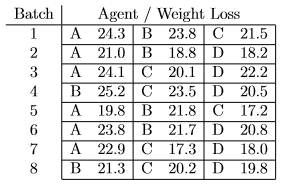
\includegraphics{prob3pic}
\end{center}


\begin{enumerate}
\item %3a
{\it What are the values of k,r,a,b and $\lambda$?}

a = 4

b = 8

$\lambda$ = 4

k = 3

r = 6

check: $4 = \frac{6(3-1)}{4-1}$

\item %3b
{\it (5.5pt) Analyze this data. Including the ANOVA table, residual plots and values, the
least squares means of the 4 cleaning processes, and the least squares estimates $\hat{\tau}_{1}$, $\hat{\tau}_{2}$,
$\hat{\tau}_{3}$, and $\hat{\tau}_{4}$.}


The model fit was:

\begin{center}
$y_{ij} = \mu + \tau_{i} + \beta_{k} + \epsilon_{ij}$ where we assume $\epsilon_{ij} \sim IIDN(0,\sigma^{2})$
\end{center}

{\bf ANOVA ANALYSIS}

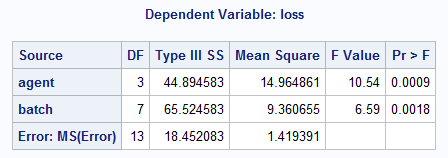
\includegraphics{prob3anova}

$H_{o}$: $\tau_{1} = ... = \tau_{4}$; $H_{a}$: at least one $\tau_{i} \neq$ the others

There is strong evidence at least one of the agents resulted in a different mean weight loss after accounting for batch ($F_{3,13}$ = 10.54, P=0.0009).

$H_{o}$: $\beta_{1} = ... = \beta_{8}$; $H_{a}$: at least one $\beta_{j} \neq$ the others

There is strong evidence at least one of the batches had a different mean weight loss that all the others after accounting for agent ($F_{7,13}$ = 6.59, P = 0.0018).

We assume the effect of agent on mean loss does not change by batch. The interaction plot supports this assumption because of the parallel lines in the empirical means.

{\bf ASSUMPTIONS}

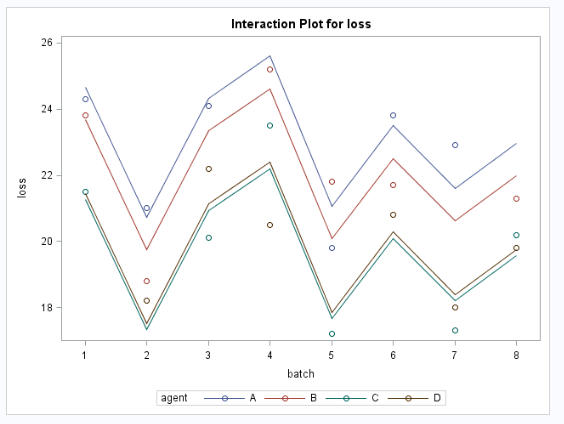
\includegraphics[scale=0.5]{prob3interaction}

The Normal Q-Q plot suggests it is reasonable to assume the residuals are distributed normally. The residuals vs. predicted plot suggests there may be slightly more variation at center predicted values than at the more extreme predicted values, possibly suggesting non-constant variance in the residuals. Randomization in the design makes independence in the residuals a reasonable assumption.

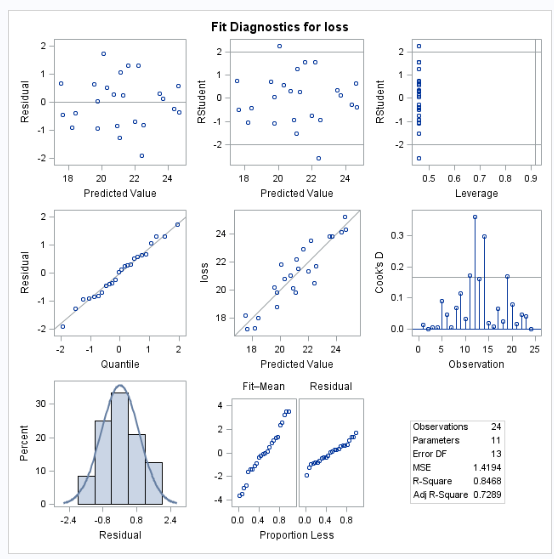
\includegraphics[scale=0.75]{prob3plots}

{\bf MEANS}

The empirical means by agent (averaged across batches) are given in the table below.

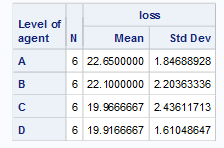
\includegraphics{prob3agent}

{\bf ESTIMATES}

The $\hat{\tau}_{i}$ estimates are given the the table below. Note that the estimate for agent D (the unconstrained $\hat{\tau}_{4}$) is set to 0, meaning that agent D is set as the baseline agent, but that the baseline mean estimate $\hat{\mu}$ does not equal the empirical mean loss for agent D given in the table above. The discrepancy is because the estimate in the table above averages overall batches while the estimate for the baseline mean is only in batch 8, and not an average effect of agent D averaged over {\it all} batches.

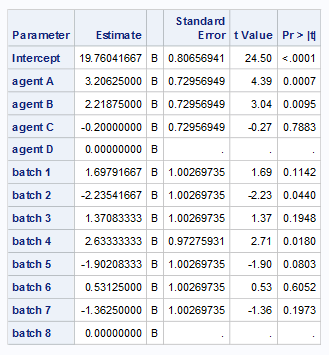
\includegraphics{prob3estimates}

\item {\it (2pt) The following table contains a table of pairwise comparisons of the least squares means. Each p-value comes from t-tests and is not adjusted for the number of pairwise comparisons. Based on these p-values and using $\alpha$ =.05, perform the Bonferroni multiple comparison procedure.}

Using Bonferroni's multiple comparison adjustment, $\alpha^{star}$ = 0.05/6 = 0.0083$\bar{3}$. Note the matrix of comparisons is symmetric, so we only need half the tests as numbers. Significant differences using Bonferonni's adjustment are: 

3 and 1

4 and 1

3 and 2



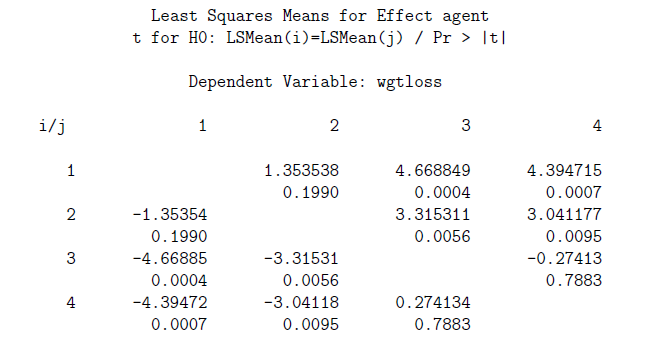
\includegraphics{prob3john}


\end{enumerate}

\item %4


\begin{enumerate}

\item %4a
(a)

There is a significant interaction effect at the $\alpha$ = 0.05 significance level ($F_{4,18}$ = 198.73, P\textless 0.0001).

Both main effects (for temperature and type) affect the mean light response. However, because we have strong evidence the effect of temperature on mean light response changes by type (and vice versa), we should only make conclusions about the effect of temperature on mean light response within a level of type (and vice versa), and not averaging over type because of the significant interaction effect.


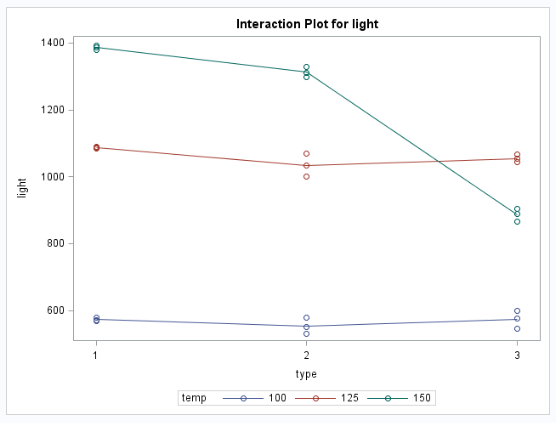
\includegraphics{prob4interaction}

(c)

There is slight curvature in the residuals vs. fitted plot which may make us question whether normality in the residuals is an assumption that is reasonably met. Of more concern is the smaller variation in the residuals seen with larger predicted values suggesting the homogeneity of variance assumption is not reasonably satisfied. Transformations to stabalize the variance should be considered and until then, results should be interpreted with caution.

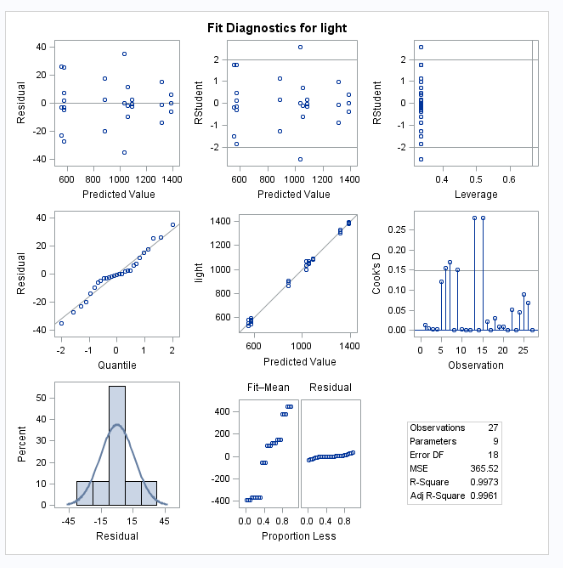
\includegraphics{prob4plots}


\item %4b

\item %4c

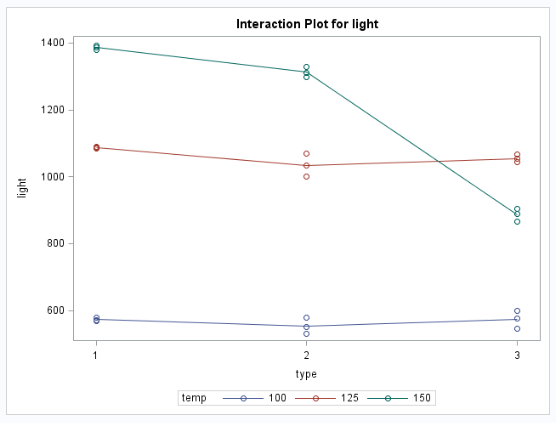
\includegraphics{prob4interaction}

The interaction plot suggests the effect of temperature 150 on mean light is different for glass types 2 and 3, but that the effect of temperatures 100 and 125 are the same for all glass types and that the effect of temperature 150 is the same for glass types 1 and 2.

\item %4d


\end{enumerate}

\end{enumerate}


\end{document}
